\chapter{Project Design}

It describes the core analysis of the requirements and the outline of the functional and non-functional aspects of the proposed CREST framework needed for proactive semantic risk detection in Neuro-Symbolic AI pipelines. Here are also the data flow diagrams at several levels. They describe the methodology and architectural components, while designing it justifies about the other solutions. Also discusses why it is taken or why which one is not. Lastly, discussed the task management of the team.  

\section{Requirement Analysis}

The most needed requirements are initially API of LLMs for forward translation and for back translation we initially decided to use another LLM, later there will be used a self made verbalizer. Also need predicate checker which runs by CPU and symbolic solver. The BERTScore package~\cite{zhang2020bertscore}, and the Z3 SMT solver bindings~\cite{demoura2008z3} are one of the core requirements here.

\subsection{Functional Requirements}

\begin{enumerate}
    \item \textbf{Forward FOL Translation:} The framework use a Large Language Model to translate each natural language premise into a First-Order Logic formula maintaining solver-compatible syntax.
    
    \item \textbf{Back-Translation and Semantic Loss Estimation:} The system does reverse translation of each generated FOL into natural language using a model distinct from the forward translator, then shows a risk score by computing semantic similarity between the back-translated text and the original premise.

    \item \textbf{Cross-Premise Predicate Consistency Checking:} The framework applies deterministic regex extraction and edit-distance comparison across all FOL formulas of a story to identify semantically similar but lexically inconsistent predicate names~\cite{thatikonda2024strategies}.

    \item \textbf{Risk-Based Routing:} The system combines two scores, one is coming from semantic loss (BERTScore) and another is from predicate risk and decide whether it should proceed to solver or not.

    \item \textbf{Error Diagnosis:} For premises scored high, the framework directs it to an LLM-as-Judge component~\cite{zheng2023judging} that returns a structured diagnosis having error type, severity, location, and feedback.

    \item \textbf{Feedback-Driven Re-translation:} The system converts the diagnosis into a feedback prompt and sends back it to the forward translator. It translates again and iterates the whole process again to pass the risk threshold.
\end{enumerate}

\subsection{Non-Functional Requirements}

\begin{enumerate}
    \item \textbf{Training-Free Operation:}  The Framework fully works at inference time, and no model fine-tuning is required. Thus, it can be directly used with any off-the-shelf Neuro-Symbolic pipeline, and the extra data and compute needed for supervised training can be ignored. 

    \item \textbf{Reproducibility:} The pipeline is designed in a way that, in every iteration of execution, we get the same result. That’s why fixed random seeds are used; intermediate output is logged in a structured way and LLM endpoint and Python dependencies exact versions are pinned there. 

    \item \textbf{Modularity:} Each part of the pipeline follows the same contract or guideline for the same input and output. As a result, the forward translator, back translator, similarity metric, predicate checker, or judge all the components can be replaced or changed individually, without changing the whole system. 

    \item \textbf{Cost Efficiency:} The Routing Mechanism is designed in a way that expensive LLMs as a judge or retranslation can only be used in high-risk or flagged cases. Thus, in the case of safe inputs, it results in less cost and latency. 
    \item  \textbf{Solver Agnosticism:} Though Z3 is used in the current implementation, this framework doesn’t rely on any specific symbolic server. By making a small change in the interface, it can be used with other FOL or SMT solvers. 
\end{enumerate}

\subsection{Data Flow Diagram}

The data flow within the CREST framework is represented across three levels of diagram. Figure~\ref{fig:dfd0} presents the Level 0 context diagram, Figure~\ref{fig:dfd1} expands the internal process structure, and Figure~\ref{fig:dfd2} details the component-level data exchange.

\begin{figure}[H]
\centering
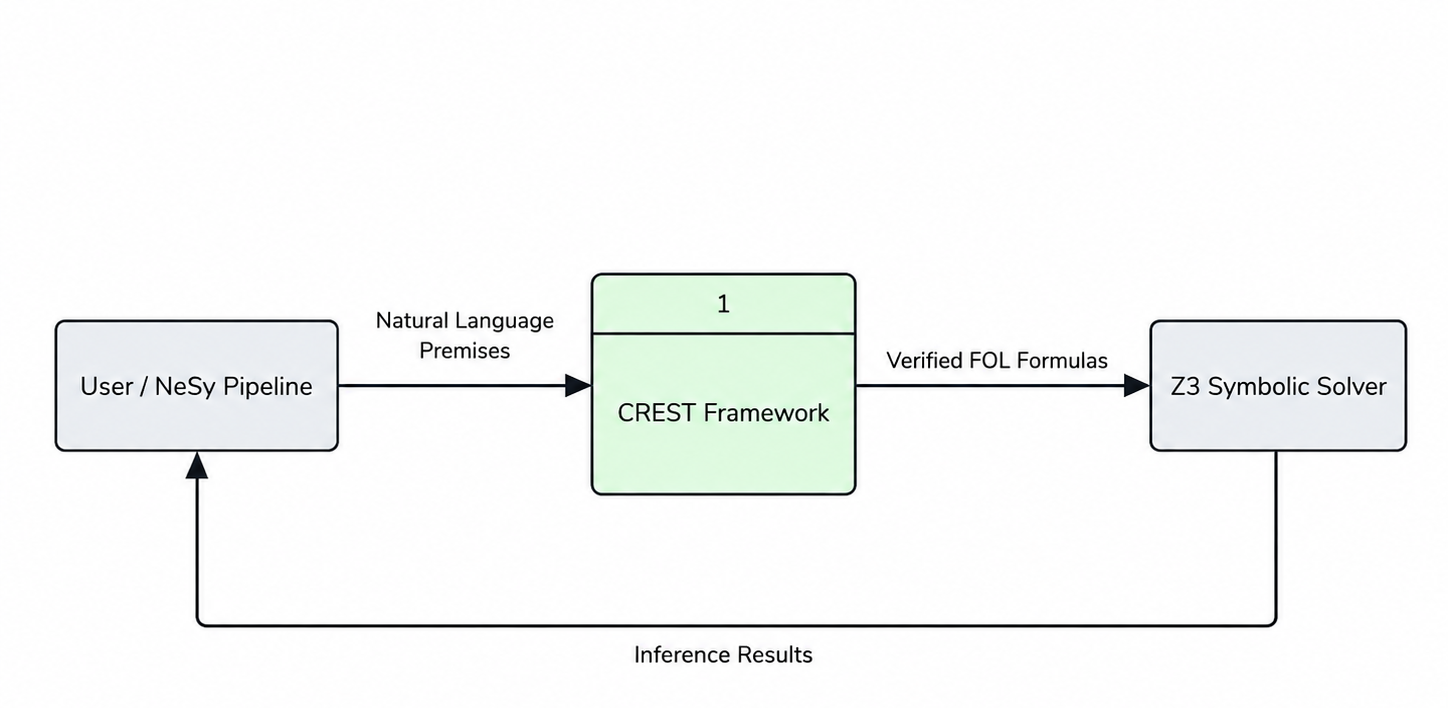
\includegraphics[width=0.85\textwidth]{./figures/dfd1.png}
\caption{DFD Level 0}
\label{fig:dfd0}
\end{figure}

\begin{figure}[H]
\centering
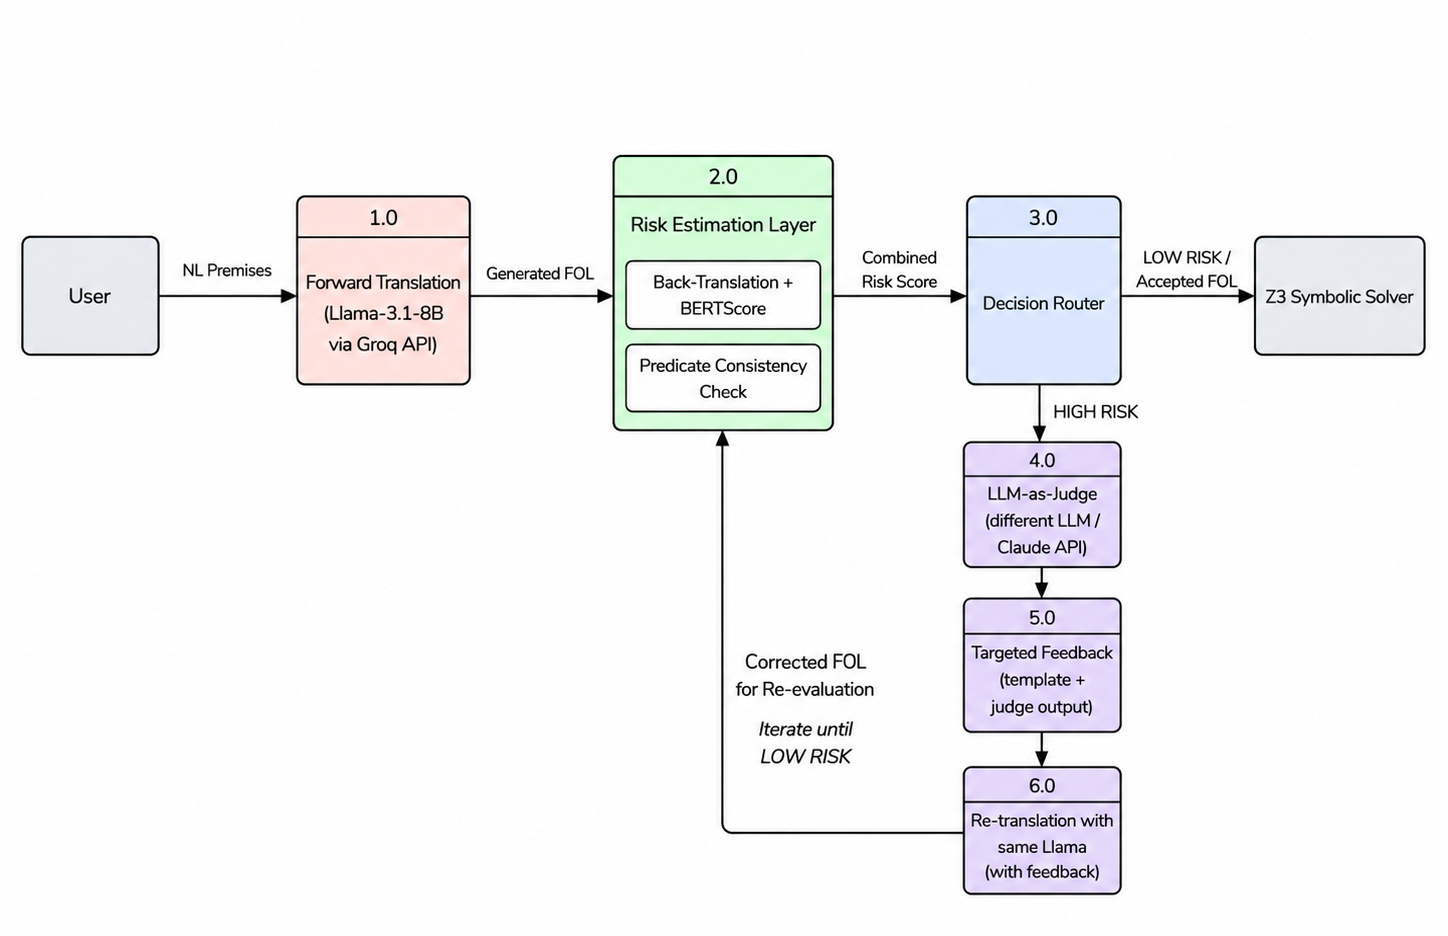
\includegraphics[width=0.95\textwidth]{./figures/dfd2.png}
\caption{DFD Level 1}
\label{fig:dfd1}
\end{figure}

\begin{figure}[H]
\centering
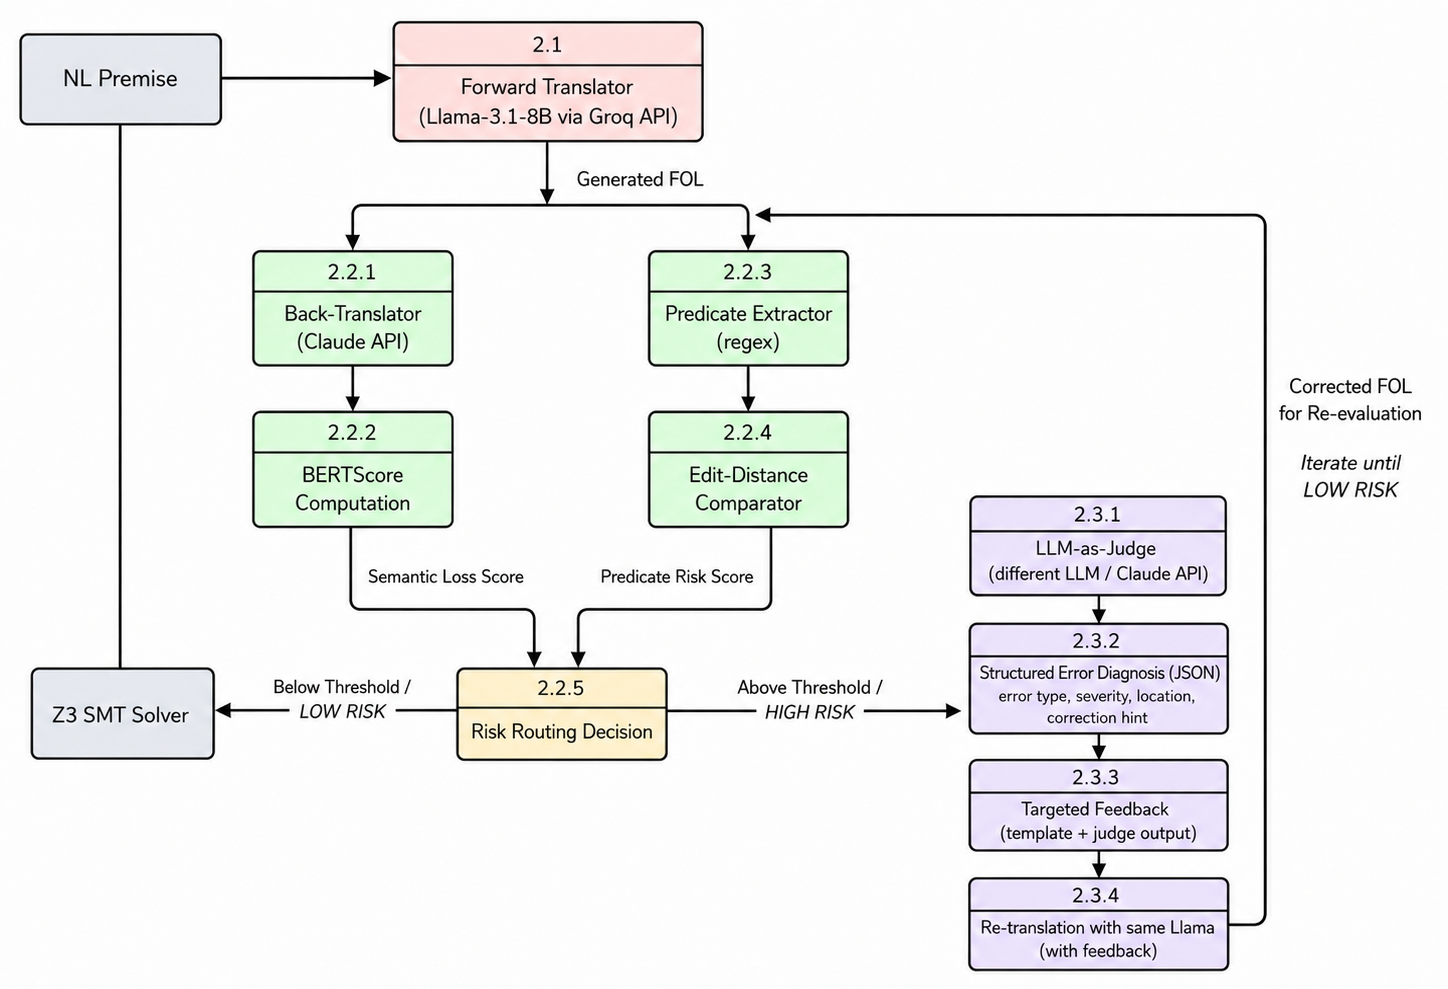
\includegraphics[width=\textwidth]{./figures/dfd3.png}
\caption{DFD Level 2}
\label{fig:dfd2}
\end{figure}

\section{Detailed Methodology and Design}

The CREST framework try to find out the fundamental safety gap at the translation limitation of Neuro-Symbolic AI pipelines. Large Language Models produce FOL translations that are syntactically valid but semantically incorrect, and symbolic theorem provers downstream have no mechanism to detect this category of error. AI logic tools do exactly what they are told. If you give them bad information, they will give you an answer that seems perfectly logical but is actually completely wrong. We call this a hidden mistake. Current fixes usually only kick in when the computer shows an error message. But this means they completely miss the bad information that the computer accepts without complaining. formulas~\cite{pan2023logiclm}, and supervised fine-tuning of dedicated verifiers, which requires annotated data~\cite{thatikonda2024strategies, yang2024harnessing}. our pipeline addresses this gap by cut off LLM-generated FOL before symbolic inference, estimating a quantitative risk score from complementary signals, diagnosing the underlying error type, and routing flagged translations through a feedback-driven correction loop. The overall architecture is depicted in Figure~\ref{fig:architecture}.

\begin{figure}[H]
\centering
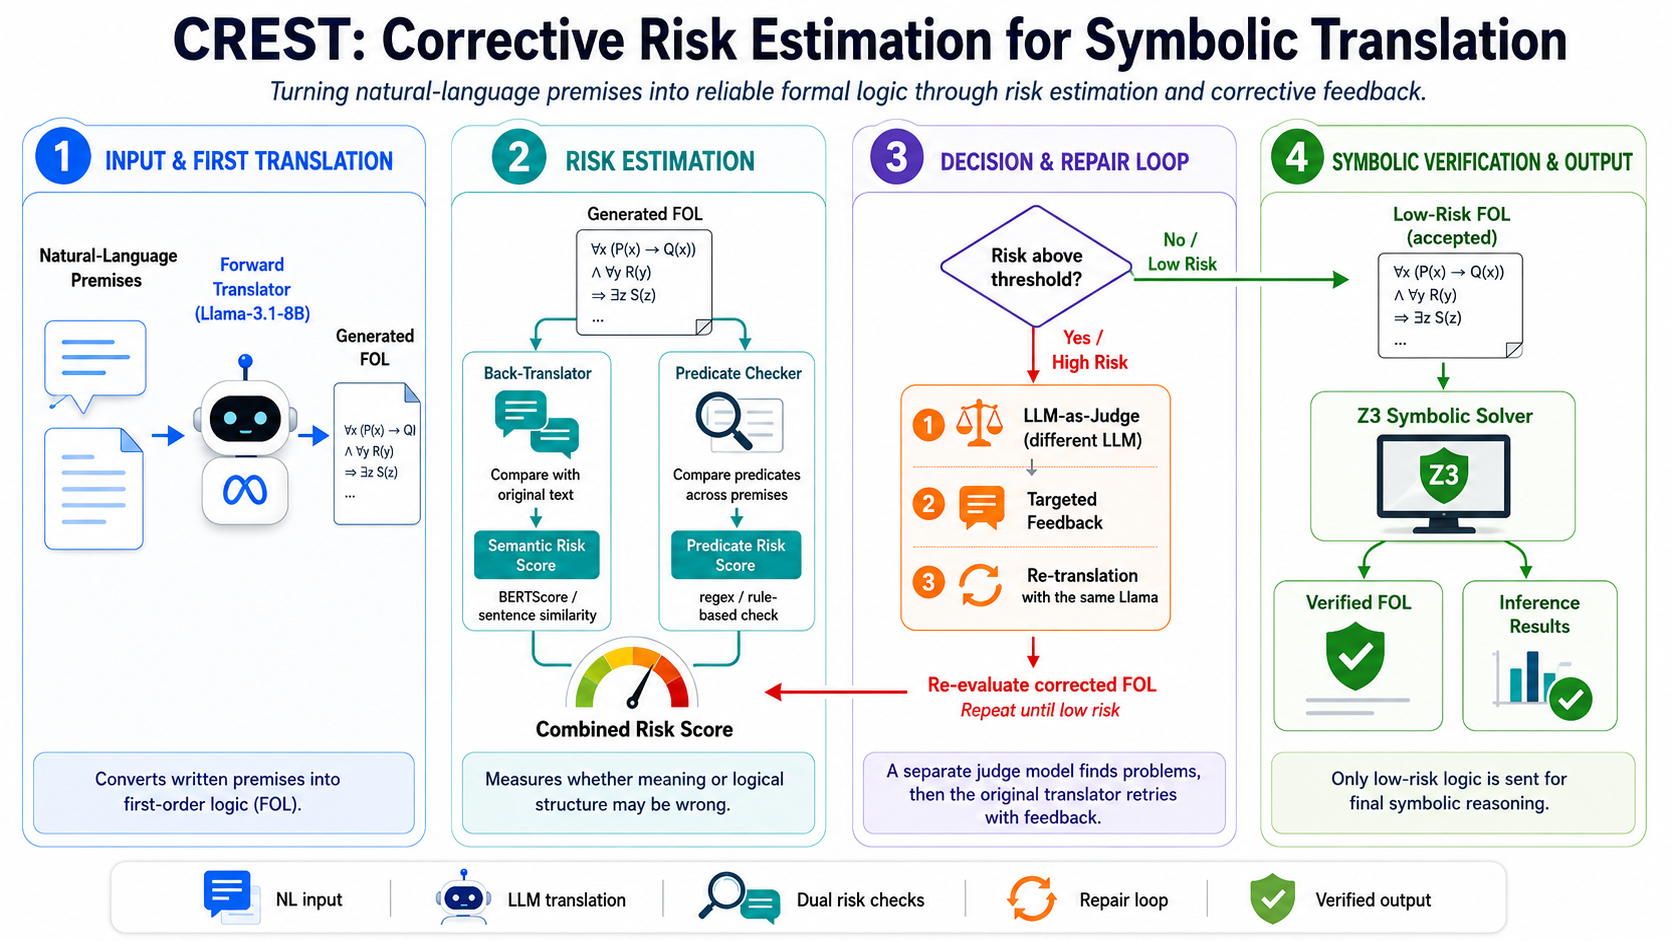
\includegraphics[width=\textwidth]{./figures/CREST.png}
\caption{Entire Architecture of the CREST Framework}
\label{fig:architecture}
\end{figure}

\subsection{Dataset}

The FOLIO benchmark~\cite{han2024folio} is used for evaluation. FOLIO is an expert-annotated dataset of 1,430 examples spanning 487 premise sets, paired with gold-standard FOL annotations that are mechanically verifiable by an FOL inference engine. We selected FOLIO because it provides ground-truth FOL at the story level rather than the isolated sentence level, enabling the cross-premise consistency analysis that constitutes a core component of the framework, and because its premises are written by human experts rather than generated from synthetic templates. For FYDP 1, a subset of 45 manually annotated premises and 20 multi-premise stories was used.In FYDP 2 will extend evaluation to the full benchmark and to ProofWriter for generalization testing.

\subsection{Forward Translation Module}

The forward translation module consumes a natural language premise and produces a corresponding FOL formula which is compatible with the Z3 solver. The module uses Llama-3.1-8B accessed through the Groq API, to balance between translation quality and inference cost. The Groq free academic tier provides sufficient token for full-scale evaluation across FOLIO. A fixed temperature of 0.1 balances deterministic behaviour with the controlled required for sampling-based analysis.

\subsection{Back-Translation and Semantic Loss Module}

The back-translation module receives the generated FOL and converts it back into natural language using the Anthropic Claude API. Using a separate model for back-translation is well-thought if the same LLM performed both directions, a systematic error such as a dropped negation could be silently reproduced in the backward direction, masking the error from comparison. The back-translated NL is compared against the original premise using BERTScore~\cite{zhang2020bertscore}, which detect meaning-level changes such as negation loss that n-gram metrics like BLEU and ROUGE systematically miss. The semantic loss signal is computed as
\[
\text{loss}_{\text{sem}} = 1 - \text{BERTScore}(\text{NL}_{\text{orig}}, \text{NL}_{\text{back}}).
\]

\subsection{Predicate Consistency Module}

The predicate consistency module operates in parallel with back-translation and analyzes the full set of FOL formulas for a story without any LLM . The module extracts predicate names from the FOL using regex-based parsing, then computes pairwise edit-distance similarity. Predicate pairs whose normalized similarity falls in the range $(0.6, 1.0)$ are flagged as suspicious, till pairs in this range typically represent the same concept expressed with minor difference such as \texttt{GoToBuilding} and \texttt{GoesToBuilding}. The module produces a binary risk flag and a quantitative predicate risk score equal to the fraction of predicates involved in suspicious pairs. The design ensures full reuse and zero API cost, complementing the neural back-translation signal.

\subsection{Risk Routing Module}

The risk routing module join the two signals and make them into a routing decision. A premise enters the corrective loop if either the semantic loss  surpass $\theta_{\text{sem}}$ or the predicate risk score exceeds $\theta_{\text{pred}}$:
\[
\text{Route to corrective loop} \iff (\text{loss}_{\text{sem}} > \theta_{\text{sem}}) \lor (\text{risk}_{\text{pred}} > \theta_{\text{pred}}).
\]
The premises that fail not either condition bypass the corrective loop and proceed directly to the symbolic solver. For balancing memory and precision on the error detection task, the thresholds are measured against the manually annotated pilot subset.

\subsection{LLM-as-Judge Module}

After receiving flagged premises along with their authentic NL,generated FOL ,back translated NL and risk score the LLM as judge module gives a structured JSON diagnostic ~\cite{zheng2023judging}. The Anthropic Claude API is used to implement the module. The judge returns four fields: error type drawn from \texttt{NEGATION\ LOSS}, \texttt{QUANTIFIER\ ERROR}, \texttt{XOR\ COLLAPSE} or \texttt{OTHER} severity rated as \texttt{CRITICAL}, \texttt{HIGH}, \texttt{MEDIUM} or \texttt{LOW}. The location of the inconsistency in the FOL and a suggestion for correction are included. The LLM judge is used instead of a rule based system because semantic errors can be unpredictable. The deterministic predicate checker covers only known errors, while the judge provides the flexibility needed to identify novel cases.

\subsection{Feedback-Driven Re-translation Module}

The re-translation module converts the judge's diagnosis into a feedback prompt using deterministic templates indexed by error type. The prompt explicitly identifies the error type and points to the affected component of the FOL, instructing the forward translator to produce a corrected version with attention to the diagnosed issue. The forward translator is re-invoked with this feedback-augmented prompt, producing a corrected FOL that is then passed to Z3. Unlike reactive self-refinement loops that operate on generic solver error messages~\cite{pan2023logiclm}, the CREST feedback mechanism uses structured semantic diagnostics, enabling targeted correction rather than generic retry.

\section{Alternative Solutions Considered}

There were other alternatives too, but those are removed because of some specific reason.
There can be used same model for back translation, but the decision is denied because, if the same model does the forward translation, it can be biased or do the same mistake silently while back translation too.
To identify semantic changes, we need some systematically sensitive metrics. That's why, surface level metric (BLEU, ROUGE) were not considered. 
Rule based error classifier was denied because, it is totally hard-coded and it can't able to find semantic differences.
Detecting consistency ~\cite{manakul2023selfcheck}  of results was also rejected because it doesn't flag error properly. Wrong results can be consistent without any feedback.

\section{Task Allocation}

The CREST framework is a hybrid model that integrates natural language processing, symbolic reasoning, semantic difference checking, and structured LLM-based evaluation. The team of five members did a deep research about this framework. Two members are allocated for the forward and back-translation pipeline, including API integration, prompt design, and request orchestration. One member is allocated for the deterministic predicate consistency module, including regex extraction, edit-distance computation, and threshold calibration. One member is allocated for the LLM-as-Judge module and feedback templates, including structured JSON prompt engineering and error taxonomy refinement. One member is responsible for the Z3 integration, the end-to-end evaluation pipeline, and the experimental analysis including manual annotation and statistical evaluation against ground truth. All team members contribute to the literature review, design discussions, and documentation, with regular  meetings to ensure consistent integration for the framework.

\section{Project Plan}

The CREST framework will be developed across two phases. In FYDP 1, three pilot experiments on the FOLIO benchmark to show the core gap, high-confidence LLM translations contain frequent semantic errors, cross premise predicate naming inconsistency is huge in LLM-generated FOL, and Z3 silently accepts semantically incorrect translations without any error signal. The deterministic Predicate Consistency Checker and Risk Scoring Framework have been partially implemented using regex-based predicate extraction and normalized edit distance, where LLM involvement is not required. In FYDP 2, the full pipeline will be deployed end-to-end across multiple benchmarks including FOLIO, ProofWriter, and PrOntoQA. The forward translator (Llama 3.1 8B) will run locally for generaing FOL, the back-translator will be replaced by a rule-based FOL-to-NL verbalizer, and the LLM-as-Judge component will be replaced by a lightweight risk-guided feedback fine tuned model which will be  trained by  using the combined risk score to make better re-translated FOL. The complete framework will be evaluated using precision, recall, and F1 on risk detection, alongside Z3 reasoning accuracy before and after CREST correction.

\section{Summary}

Chapter 3 explained how the CREST system is built, how it works, and who on the team is doing what. It started by listing exactly what the system needs to do to catch hidden errors early. We used clear diagrams to show step-by-step how data enters, moves through, and leaves the system. The chapter also broke down every single part of the tool like the translators, error checkers, and the AI judge that helps fix mistakes. We even explained why we rejected other design ideas. Finally, we listed the jobs for our five team members, giving us a clear plan to build and test everything in the next phase (FYDP 2).